\documentclass{beamer}

% For more themes, color themes and font themes, see:
% http://deic.uab.es/~iblanes/beamer_gallery/index_by_theme.html
%
\mode<presentation>
{
  \usetheme{Madrid}       % or try default, Darmstadt, Warsaw, ...
  \usecolortheme{beaver} % or try albatross, beaver, crane, ...
  \usefonttheme{serif}    % or try default, structurebold, ...
  \setbeamertemplate{navigation symbols}{}
  \setbeamertemplate{caption}[numbered]
} 

\usepackage{tikz}
\usetikzlibrary{decorations.markings,angles}
\usepackage{tikz-3dplot} 

\usepackage{amsmath}


\begin{document}

\title[Two-fluid simulations]  
{Two-fluid simulations of solar partially ionized atmosphere }

\begin{frame}
\maketitle
\end{frame}


\usebackgroundtemplate{%
  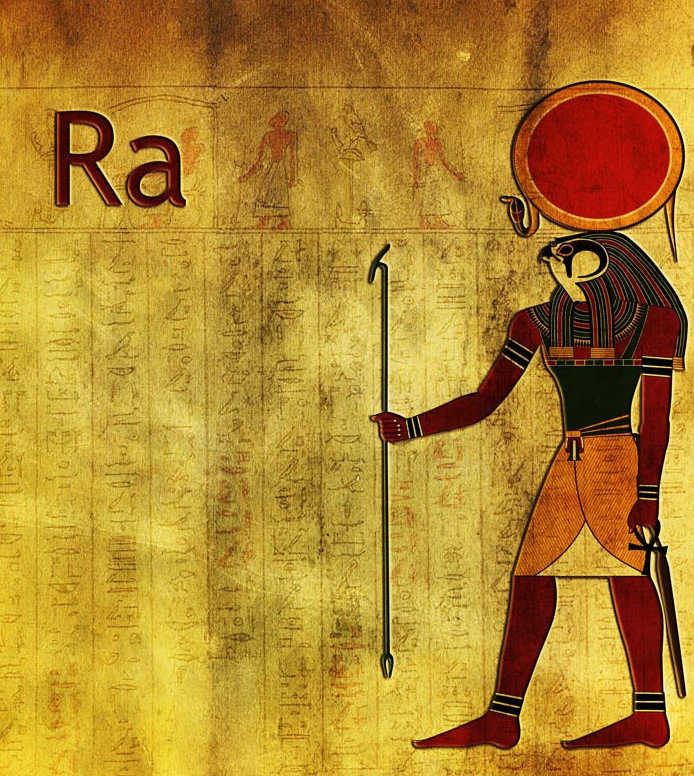
\includegraphics[width=\paperwidth,height=\paperheight]{ra.png}} 


\begin{frame}{Ever fascinating sun}
\vspace*{3cm}
\begin{figure}[H]
 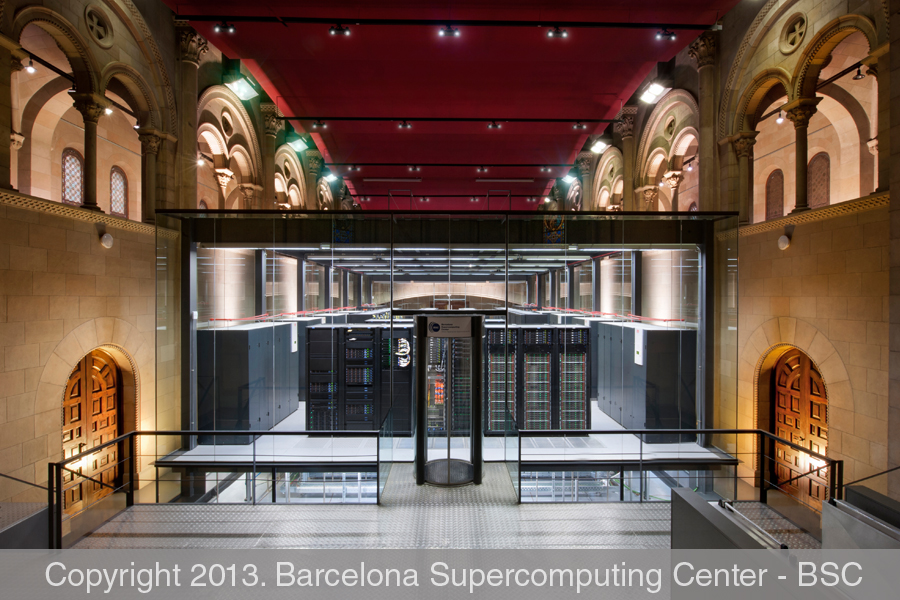
\includegraphics[scale=0.2]{mn.jpg} \hspace*{12cm}
\end{figure}
\end{frame}

\usebackgroundtemplate{ }  

\begin{frame}{Studying the sun(observations)}
\begin{itemize}
\item The first written record of sunspots was made by Chinese astronomers around 800 B.C
\item 1982 years before the first drawing

\begin{figure}[H]
 \centering
 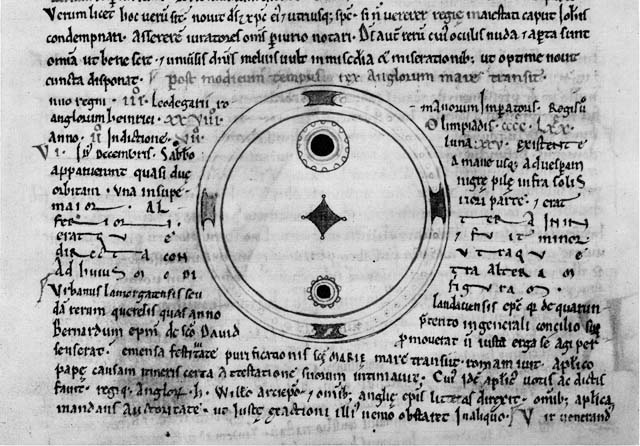
\includegraphics[scale=0.5]{jwex.jpg}
  \caption{The earliest known drawing of sunspots appears in The Chronicle of John of Worcester 
	and predates the invention of the telescope by almost 500 years. 
	The sunspot was recorded in medieval England in 1182, according to astronomer 
	F. Richard Stephenson at the University of Durham. }
\end{figure}


\end{itemize}

\end{frame}

\begin{frame}{Studying the sun(observations)}
\begin{figure}[H]
 \centering
 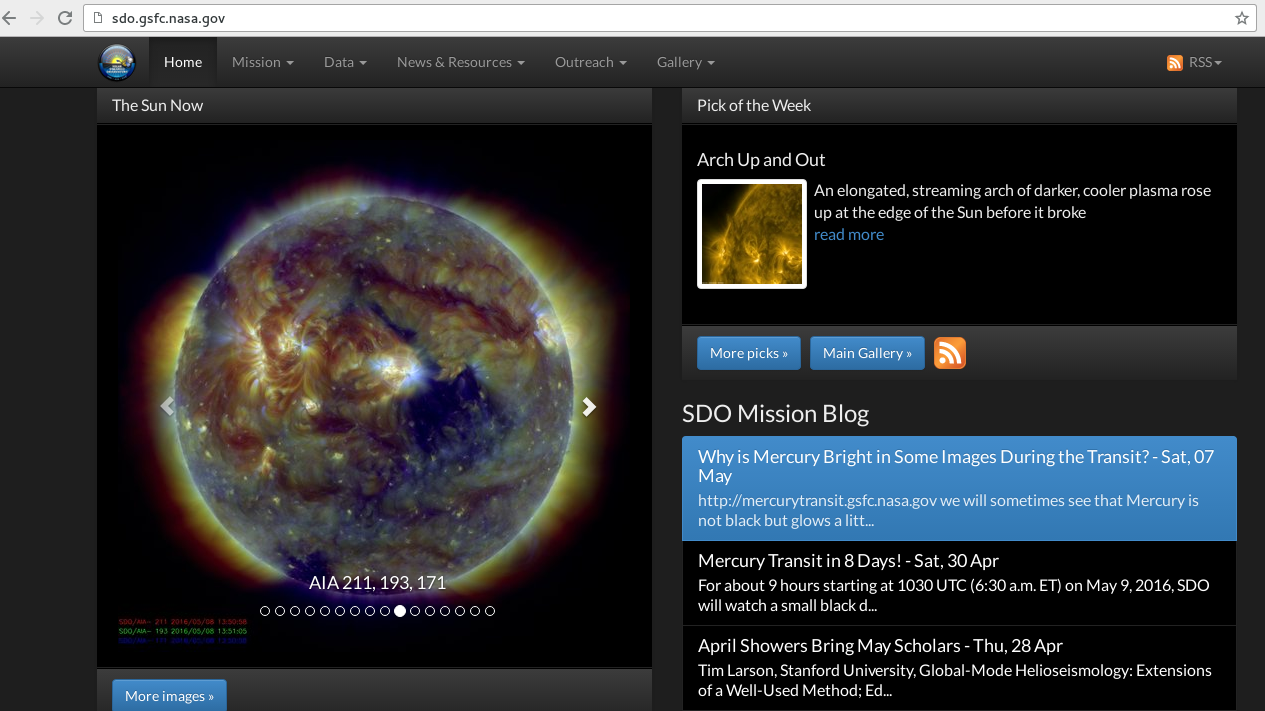
\includegraphics[scale=0.25]{sdo.png}
  \caption{SDO space telescope live images of the sun in several wavelengths}
\end{figure}
\end{frame}

\begin{frame}{Mysteries of the sun}
\begin{itemize}
\item solar cycle
\begin{figure}[H]
 \centering
 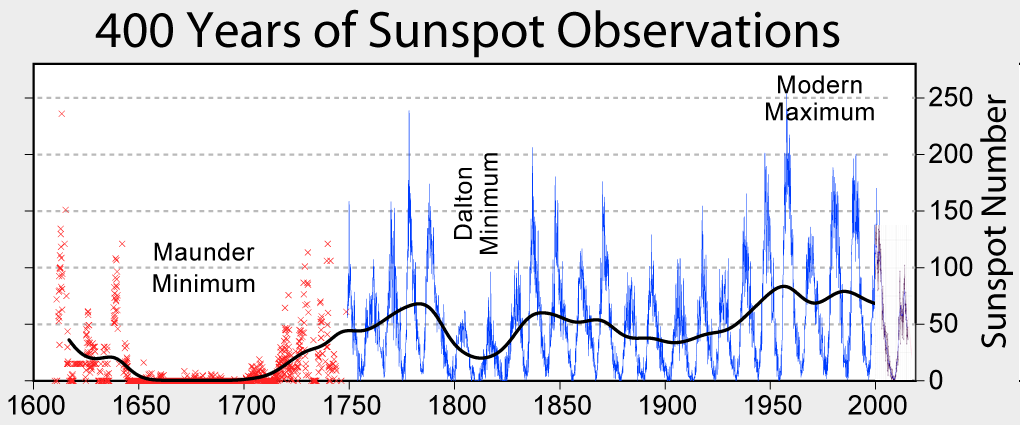
\includegraphics[scale=0.4]{cycle.png}
  \caption{solar magnetic activity cycle is the nearly periodic 11-year change in the Sun's activity}
\end{figure}
\end{itemize}
\end{frame}



\begin{frame}{Mysteries of the sun}

\begin{itemize}
\item the mechanism of the generation of 
a magnetic field thousands times stronger 
than on earth concentrated in spots as large as earth (the sunspots)
\item coronal heating: above the photosphere at around 6000 K the temperature rises abruptly at over 1 million degrees 
\end{itemize}

\end{frame}


\begin{frame}{Studying the sun(theoretical models)}
Sun as a plasma(a gas containing neutral and charged particles, but globally electrically neutral with collective behaviour)
\begin{itemize}
\item main sequence star burning hydrogen into helium into its core
\item the sun atmosphere is composed mainly of H and He (the proportion of number of atoms H:He is 10:1 and the metallicity estimated Z = 0.0122)
\item neutral atoms in the photosphere  start to become ionized in the chromosphere where temperature starts to rise and  
are fully ionized in the corona  
\end{itemize}
Plasma models
\begin{itemize}
\item fluid mechanics equations derived (in statistical physics) from Boltzmann equation 
for variables like density, pressure and velocity
\item induction equation derived from Maxwell equations and Ohm law for the evolution of the magnetic field
\end{itemize}

\end{frame}

\begin{frame}{Plasma models}
\begin{itemize}
\item system of first order non linear partial differential equations which must be integrated in time
\item Approximations:
\begin{itemize}
\item MHD: all the particles are considered as a whole. Assumption: strongly collisional plasma. A system of 8 unknown variables
($p,\rho,v_x,v_y,v_z,B_x,B_y,B_z$)
\item 2-fluid: Neutral particles do not feel electromagnetic forces and may move  differently from charged particles so collision rates between 
charged particles and neutral particles may not be the same like inside one specie. 
We consider the fluid variables ($p,\rho,v_x,v_y,v_z$) different for charged and neutral particles. A system of 13 unknown variables.
\item furthermore we could split the charges into ions and electrons as sometimes forces act differently on them
\end{itemize}
\end{itemize}
\end{frame}
\end{document}
